% Use xelatex to generate a pdf file of this presentation

\documentclass{beamer}
% \usepackage{roboto}
\usepackage[english]{babel}
\usetheme{Copenhagen}

% Simple way to put a code listing to the slide
\usepackage{listings}

\usepackage{tikz}
\usetikzlibrary{positioning,calc,arrows.meta,decorations.pathreplacing}
\usepackage{pgfplots}
\pgfplotsset{compat=1.18}
\usepackage{graphicx}
\usepackage{qrcode}
\usepackage{booktabs}
\usepackage{amsmath}
\usepackage{amssymb}

% Blocks settings
\setbeamerfont{block title}{size=\tiny}
\setbeamertemplate{navigation symbols}{}

%Information to be included in the title page:
\title{Polymorphic Reference Resolution}
\subtitle{Bottlenecks in N-Way LEFT JOIN Queries}
\author{Andrei Lepikhov}
\institute{pgEdge}
\date{2026}

% Add page numbers in the footnote
\expandafter\def\expandafter\insertshorttitle\expandafter{%
  \insertshorttitle\hfill%
  \insertframenumber\,/\,\inserttotalframenumber}

\definecolor{lightlightgray}{gray}{0.9}
\definecolor{pgblue}{HTML}{336791}
\definecolor{pgorange}{HTML}{E8781A}

% Default listing format
\lstset{language=sql, frame=none, tabsize=2, identifierstyle=\color{black},
  showspaces=false, showtabs=false, showstringspaces=false,
  columns=fullflexible, % Restore default spaces between letters
  basicstyle=\rmfamily\scriptsize,
  stringstyle=\color{purple},
  keywordstyle=\bfseries\color{green!40!black},
  numberstyle=\tiny\color{gray},
  morekeywords={COALESCE,PUBLICATION,SUBSCRIPTION,CONNECTION,WITH,COPY,FORMAT,
    SERIAL,VARCHAR,REFERENCES,EXISTS,ANALYZE,BUFFERS}}

% -----------------------------

\begin{document}

% THEORETICAL BACKGROUND (not shown on slides):
%
% A "discriminated foreign key" encodes a polymorphic reference as two columns:
%   - discriminator (item_type): identifies the target table
%   - polymorphic FK (item_id): identifies the row within that table
%
% No single FOREIGN KEY constraint can span multiple target tables, so the
% database treats item_id as an ordinary integer.  To resolve the reference,
% the query must LEFT JOIN against every possible target table, guarded by
% the discriminator value.
%
% The pattern arises in two forms:
%   1. Polymorphic associations (Rails, Django) -- no referential integrity
%   2. Joined-table inheritance (Hibernate JOINED) -- with referential integrity
% Both produce the same query shape.

% THEORY: Resolution query structure
%
% For each row, the query LEFT JOINs against every candidate target table.
% The discriminator predicate in each join condition ensures that at most one
% join produces a match; the remaining N-1 produce NULLs.  COALESCE collapses
% the results.
%
% Three structural invariants distinguish this from arbitrary outer joins:
%   1. Mutual exclusion: discriminator predicates are pairwise disjoint
%   2. Inner-key uniqueness: join key on each target is PK/unique
%   3. Column-usage constraint: target columns only appear inside COALESCE/CASE

\begin{frame}[fragile]\frametitle{The Query}
\begin{lstlisting}
SELECT
    ol.id,
    COALESCE(p.name, g.name, s.name) AS item_name
FROM order_lines ol
  LEFT JOIN products p
    ON ol.item_type = 'product' AND ol.item_id = p.id
  LEFT JOIN gift_cards g
    ON ol.item_type = 'gift_card' AND ol.item_id = g.id
  LEFT JOIN subscriptions s
    ON ol.item_type = 'subscription' AND ol.item_id = s.id
WHERE EXISTS (
  SELECT 1 FROM orders o
  WHERE o.id = ol.order_id AND o.placed_at >= 2024\−01\−01)
ORDER BY ol.popularity
LIMIT 100
\end{lstlisting}
\end{frame}

% THEORETICAL BACKGROUND: Execution cost amplifiers
%
% The base cost of the polymorphic pattern is O(M * N) probes, of which
% only O(M) are useful.  Several real-world factors amplify this cost
% beyond the simple model.  We enumerate them here as "amplifiers" --
% conditions that multiply the already-wasteful base cost.
%
% Amplifier 1: Base-table growth (M growth)
%
%   The total number of probes (fruitless + useful) is M * N.
%   As M grows, the absolute number of fruitless probes grows linearly.
%   For nested-loop with index probes, each fruitless probe is a B-tree
%   traversal.  At M = 10^6 and N = 10, that's 9 * 10^6 wasted B-tree
%   lookups.  At M = 10^8, it's 9 * 10^8.
%
%   Crucially, the USEFUL work also grows linearly with M (you still need
%   M matching probes), so the waste RATIO (N-1)/1 is constant.  But the
%   absolute cost matters: 9 * 10^8 B-tree lookups can dominate wall-clock
%   time even when each individual lookup is microseconds.
%
%   The inner-side B-tree height h grows logarithmically with the target
%   table size |T_k|, but |T_k| is typically much smaller than M (each
%   target table holds only one subtype's rows).  So B-tree depth is
%   usually 2-4 and does not contribute much to growth.  The dominant
%   factor is the sheer count of probes: M * (N-1).
%
% Amplifier 2: Unindexed base-table filter (sequential scan + full probe chain)
%
%   When the query includes a WHERE clause on the base table (e.g., a date
%   range, a status filter, or an EXISTS subquery), the ideal plan pushes
%   this filter down to the base-table scan so that only qualifying rows
%   enter the LEFT JOIN chain.
%
%   If the filter column has an index, the base scan can use an index scan
%   or bitmap scan, reading only the qualifying rows.  The number of rows
%   entering the LEFT JOIN chain is s * M (where s is the filter selectivity),
%   and the total probe count drops to s * M * N.
%
%   But if there is no index on the filter column, the base table is
%   sequentially scanned.  Two sub-cases arise:
%
%   (a) Filter pushed below joins (good case): The sequential scan reads
%       all M rows but applies the filter immediately, so only s * M rows
%       enter the join chain.  The cost is: seqscan(M) + s * M * N probes.
%       The seqscan adds O(M) I/O but the probe count is still reduced.
%
%   (b) Filter NOT pushed below joins (bad case -- e.g., EXISTS displaced
%       above the join chain due to join_collapse_limit): All M rows enter
%       the join chain, producing M * N probes.  The filter is applied
%       AFTER the joins, discarding (1-s) * M rows that have already
%       performed N fruitless probes each.  Total wasted probes:
%       (1-s) * M * N + M * (N-1) ~= M * N for small s.
%
%   In practice, case (b) is common with the polymorphic pattern because
%   the high relation count (N+1 or more) frequently exceeds
%   join_collapse_limit, preventing the planner from pushing semi-joins
%   or filters into optimal positions.
%
% Amplifier 3: Target-type count growth (N growth)
%
%   Adding a new subtype to the data model adds a new LEFT JOIN to the
%   resolution query.  This has three compounding effects:
%
%   (a) Direct cost: one more fruitless probe per base row (linear in N)
%   (b) join_collapse_limit cliff: at N+1 > limit, the planner loses
%       join reordering ability (step function)
%   (c) Estimation error compounding: one more join multiplies the
%       cumulative cardinality estimation error (exponential in N)
%
%   The transition from N=7 to N=8 can cause a discontinuous jump in
%   query time because it crosses the default join_collapse_limit of 8,
%   simultaneously triggering (b) and potentially (c).
%
% Amplifier 4: Skewed discriminator distribution
%
%   If the discriminator distribution is highly skewed -- e.g., 95% of rows
%   have item_type = 'product' and the remaining 5% are spread across 9
%   other types -- then for 95% of base rows, 9 out of 10 probes are
%   fruitless.  The "average" cost per row is:
%     0.95 * (1 useful + 9 fruitless) + 0.05 * (1 useful + 9 fruitless)
%     = 1 useful + 9 fruitless per row (same as uniform!)
%
%   The waste ratio is the same regardless of skew: always (N-1) fruitless
%   per row.  However, skew affects the OPTIMIZER's behavior:
%
%   - For the dominant type ('product'), a hash join might be efficient
%     because s_product * M rows probe products, justifying the build cost.
%   - For rare types, the hash table build cost is amortized over very few
%     matching probes, making nested-loop + index more efficient.
%   - The optimizer must choose ONE method per join, and cannot adapt
%     per-row to the discriminator value.
%
%   Skew also means that if the optimizer could somehow "skip" non-matching
%   joins, the benefit would be largest for the dominant type: 95% of rows
%   would skip 9 joins, saving 0.95 * M * 9 probes.

\begin{frame}\frametitle{Typical optimiser choices}
\begin{itemize}
  \item NestLoop LEFT JOIN type because of PK index scan on the inner side
\end{itemize}
\end{frame}


\begin{frame}\frametitle{Query Plan Tree}
\begin{center}
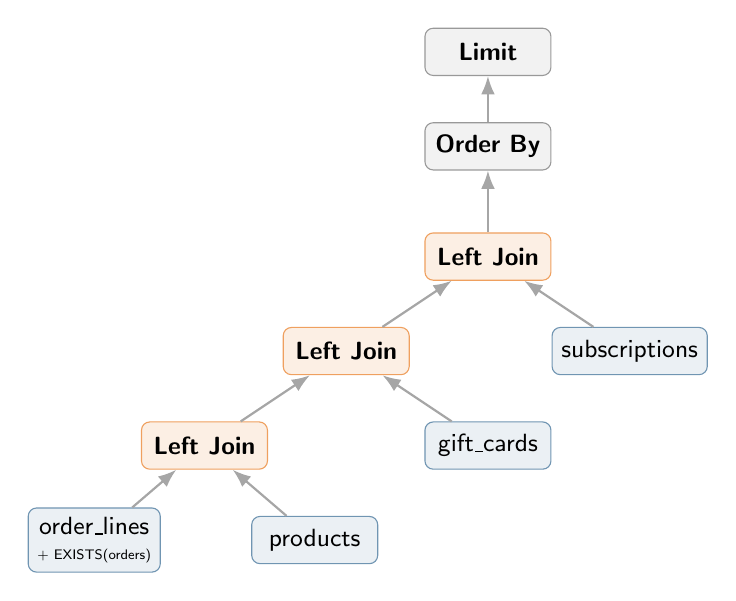
\begin{tikzpicture}[
  joinnode/.style={draw=pgorange!70, rounded corners=3pt, fill=pgorange!12,
               minimum height=0.6cm, minimum width=1.6cm,
               align=center, font=\sffamily\small},
  tbl/.style={draw=pgblue!70, rounded corners=3pt, fill=pgblue!10,
              minimum height=0.6cm, minimum width=1.6cm,
              align=center, font=\sffamily\small},
  op/.style={draw=black!40, rounded corners=3pt, fill=black!5,
             minimum height=0.6cm, minimum width=1.6cm,
             align=center, font=\sffamily\small},
  edge/.style={thick, -Latex, gray!70},
]

% Row 0: Limit
\node[op] (limit) at (0, 0) {\textbf{Limit}};

% Row 1: Order By
\node[op] (orderby) at (0, -1.2) {\textbf{Order By}};

% Row 2: Left Join 3
\node[joinnode] (lj3) at (0, -2.6) {\textbf{Left Join}};

% Row 3: Left Join 2 + subscriptions
\node[joinnode] (lj2) at (-1.8, -3.8) {\textbf{Left Join}};
\node[tbl] (t3) at (1.8, -3.8) {subscriptions};

% Row 4: Left Join 1 + gift_cards
\node[joinnode] (lj1) at (-3.6, -5.0) {\textbf{Left Join}};
\node[tbl] (t2) at (0, -5.0) {gift\_cards};

% Row 5: order_lines + products
\node[tbl, align=center] (base) at (-5.0, -6.2)
  {order\_lines\\[-2pt]{\tiny\textsf{+ EXISTS(orders)}}};
\node[tbl] (t1) at (-2.2, -6.2) {products};

% Edges (arrows point upward = data flow direction)
\draw[edge] (orderby) -- (limit);
\draw[edge] (lj3) -- (orderby);
\draw[edge] (lj2) -- (lj3);
\draw[edge] (t3) -- (lj3);
\draw[edge] (lj1) -- (lj2);
\draw[edge] (t2) -- (lj2);
\draw[edge] (base) -- (lj1);
\draw[edge] (t1) -- (lj1);

\end{tikzpicture}
\end{center}
\end{frame}

\begin{frame}\frametitle{Main Execution Cost Amplifiers}
\begin{itemize}
  \item Base table (\texttt{order\_lines}) growth
  \item Ordering/grouping column of the base table not covered by an index
  \item Growth in the number of LEFT JOINs (target types)
  \item Unstable placement of the EXISTS filter
\end{itemize}
\end{frame}

% THEORY: Query plan structure and amplifier mapping
%
% The plan tree below represents the "bad" case -- what the planner produces
% when join_collapse_limit is exceeded and no index covers the ORDER BY column.
%
% Plan tree (bottom-up execution):
%
%   Limit 100
%     Sort (ol.popularity)            -- must consume ALL input before emitting
%       Semi Join (orders)            -- displaced: filters AFTER all LEFT JOINs
%         NestLoop Left Join          -- subscriptions
%           NestLoop Left Join        -- gift_cards
%             NestLoop Left Join      -- products
%               Seq Scan order_lines  -- M rows, no early termination
%             Index Scan products_pkey
%           Index Scan gift_cards_pkey
%         Index Scan subscriptions_pkey
%       Index Scan orders (placed_at)
%
% Where each amplifier applies:
%
%   Amplifier 1 (base table growth): Seq Scan on order_lines produces M rows.
%   Every row propagates through the entire LEFT JOIN chain.  Doubling M
%   doubles the total number of probes.
%
%   Amplifier 2 (N growth): The LEFT JOIN chain has N nested-loop nodes.
%   Each base row visits all N inner sides.  Adding one more target type
%   adds one more nested-loop node and one more fruitless probe per row.
%   At N+1 > join_collapse_limit, the planner also loses reordering freedom.
%
%   Amplifier 3 (no index on sort column): The Sort node is a blocking
%   operator -- it must consume ALL input rows before it can emit any.
%   This defeats the Limit node above it: even though only 100 rows are
%   needed, all M rows must pass through the LEFT JOIN chain and the
%   Semi Join before the Sort can begin.  With an index on popularity,
%   the planner could use an index-ordered scan on order_lines, feed rows
%   into the LEFT JOIN chain one at a time in popularity order, and stop
%   after 100 rows -- reducing total probes from M*N to ~100*N.
%
%   Amplifier 4 (EXISTS displacement): The Semi Join sits above the LEFT
%   JOIN chain instead of below it.  All M rows pass through N LEFT JOINs
%   first; only then does the Semi Join discard non-matching rows.  If
%   EXISTS selectivity is s, the useful work is s*M*N probes, but the
%   actual work is M*N probes -- a factor of 1/s wasted.

% Visual style follows industrial convention (pgAdmin, PEV2, PGConf talks):
%   - Rounded rectangles with semantic color coding
%   - Blue/teal: scan/table nodes; Orange: join nodes; Gray: other operators
%   - Sans-serif bold operator name
%   - Clean arrows with arrowheads (data flows upward)
%   - Logical operators (ORDER BY, not Sort; Left Join, not NestLoop)

% THEORY: Base-table growth amplifier
%
% When the base table grows from M to M', every edge on the left spine
% of the plan tree carries proportionally more rows.  Each Left Join is
% a nested loop: for every outer row it probes the inner side.  The inner
% side produces at most 1 match (PK uniqueness), so output rows = input
% rows = M.  The LEFT JOIN never reduces the row count.
%
% Row counts along the left spine:
%   base -> LJ1: M rows
%   LJ1 -> LJ2: M rows (LEFT JOIN preserves all outer rows)
%   LJ2 -> LJ3: M rows
%   LJ3 -> Order By: M rows
%   Order By -> Limit: M rows (blocking: must consume all before emitting)
%
% Each Left Join also drives M probes into its inner (right) child.
% With N=3 joins, total inner-side probes = 3*M.
% Useful probes (matching) = M.  Fruitless probes = (N-1)*M = 2*M.
%
% Doubling M doubles every number on every edge.

\begin{frame}\frametitle{Worst case: base table growth + no index scan}
\vspace{-2mm}
\begin{center}
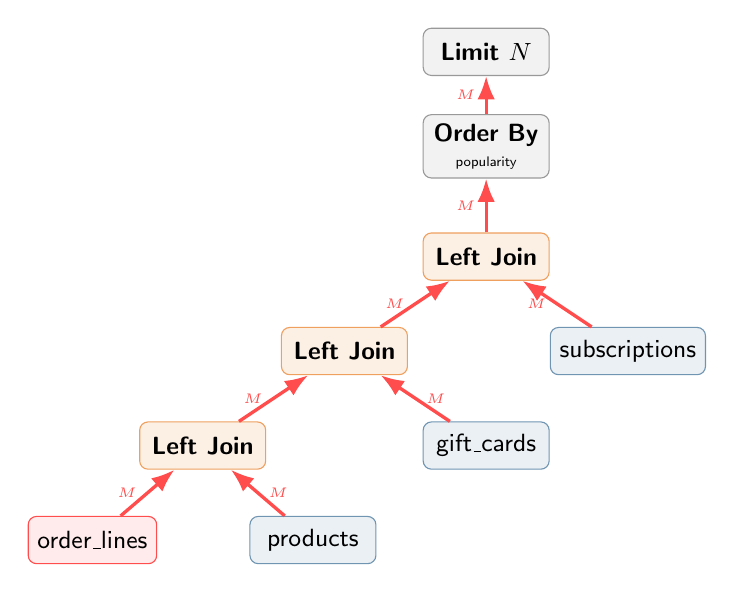
\begin{tikzpicture}[
  joinnode/.style={draw=pgorange!70, rounded corners=3pt, fill=pgorange!12,
               minimum height=0.6cm, minimum width=1.6cm,
               align=center, font=\sffamily\small},
  tbl/.style={draw=pgblue!70, rounded corners=3pt, fill=pgblue!10,
              minimum height=0.6cm, minimum width=1.6cm,
              align=center, font=\sffamily\small},
  op/.style={draw=black!40, rounded corners=3pt, fill=black!5,
             minimum height=0.6cm, minimum width=1.6cm,
             align=center, font=\sffamily\small},
  edge/.style={thick, -Latex, gray!70},
  hot/.style={very thick, -Latex, red!70},
  rows/.style={font=\sffamily\tiny\bfseries, text=red!70},
]

% Row 0: Limit
\node[op] (limit) at (0, 0) {\textbf{Limit $N$}};

% Row 1: Order By (show sort attribute — key to this amplifier)
\node[op] (orderby) at (0, -1.2) {\textbf{Order By}\\[-2pt]{\tiny popularity}};

% Row 2: Left Join 3
\node[joinnode] (lj3) at (0, -2.6) {\textbf{Left Join}};

% Row 3: Left Join 2 + subscriptions
\node[joinnode] (lj2) at (-1.8, -3.8) {\textbf{Left Join}};
\node[tbl] (t3) at (1.8, -3.8) {subscriptions};

% Row 4: Left Join 1 + gift_cards
\node[joinnode] (lj1) at (-3.6, -5.0) {\textbf{Left Join}};
\node[tbl] (t2) at (0, -5.0) {gift\_cards};

% Row 5: order_lines (highlighted) + products
\node[tbl, draw=red!70, fill=red!8, align=center] (base) at (-5.0, -6.2)
  {order\_lines};
\node[tbl] (t1) at (-2.2, -6.2) {products};

% Hot edges (left spine -- all carry M rows)
\draw[hot] (base) -- node[rows, left, pos=0.5] {$M$} (lj1);
\draw[hot] (lj1) -- node[rows, left, pos=0.5] {$M$} (lj2);
\draw[hot] (lj2) -- node[rows, left, pos=0.5] {$M$} (lj3);
\draw[hot] (lj3) -- node[rows, left, pos=0.5] {$M$} (orderby);
\draw[hot] (orderby) -- node[rows, left, pos=0.5] {$M$} (limit);

% Inner-side edges (each probed M times)
\draw[hot] (t1) -- node[rows, right, pos=0.5] {$M$} (lj1);
\draw[hot] (t2) -- node[rows, right, pos=0.5] {$M$} (lj2);
\draw[hot] (t3) -- node[rows, left, pos=0.5] {$M$} (lj3);

% Cold edges -- none; all edges are affected

\end{tikzpicture}
\end{center}
\vspace{-2mm}
{\small Every edge carries $M$ rows. Doubling $M$ doubles number of probes on the inner side.}
\end{frame}


% From pgsql-hackers thread (Dec 2024):
% "Do not scan index in right table if condition for left join
%  evaluates to false using columns in left table"
%
% Tom Lane: "One could imagine that we split up the join filter
% conditions into 'depends on RHS' and 'doesn't depend on RHS'
% subsets, and make the nestloop plan node evaluate the latter set
% only once per LHS row, and then skip the inner-side scan when
% that condition fails."
%
% Andres Freund's idea: push the "doesn't depend on RHS" subset into
% a one-time Result filter node atop the RHS subtree.  No new executor
% machinery needed — the existing Result node already supports one-time
% filter evaluation.  When the filter is false, Result returns zero rows
% and the inner-side scan is never launched.
%
% Current behavior:
%   NestLoop Left Join
%     Join Filter: (p.dtype = 'B')   ← evaluated AFTER inner scan
%     → parent (outer)
%     → Index Scan child (inner)     ← always executed
%
% Andres's proposed behavior:
%   NestLoop Left Join
%     → parent (outer)
%     → Result                       ← one-time filter: p.dtype = 'B'
%       → Index Scan child (inner)   ← skipped when Result filter is false

\begin{frame}\frametitle{Concept: Result Filter (from pgsql-hackers)}
\vspace{-1mm}
\begin{columns}[T]

% Left column: CURRENT behavior
\begin{column}{0.48\textwidth}
\centering
{\small\textbf{Current: probe, then filter}}
\vspace{2mm}

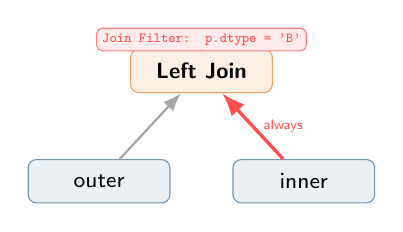
\begin{tikzpicture}[
  joinnode/.style={draw=pgorange!70, rounded corners=3pt, fill=pgorange!12,
               minimum height=0.55cm, minimum width=1.8cm,
               align=center, font=\sffamily\footnotesize},
  tbl/.style={draw=pgblue!70, rounded corners=3pt, fill=pgblue!10,
              minimum height=0.55cm, minimum width=1.8cm,
              align=center, font=\sffamily\footnotesize},
  edge/.style={thick, -Latex, gray!70},
  hot/.style={very thick, -Latex, red!70},
  filt/.style={font=\sffamily\tiny, text=red!70},
]

\node[joinnode] (lj) at (0, 0) {\textbf{Left Join}};

\node[tbl] (outer) at (-1.3, -1.4) {outer};
\node[tbl] (inner) at (1.3, -1.4) {inner};

\draw[edge] (outer) -- (lj);
\draw[hot] (inner) -- node[filt, right, pos=0.5] {\textsf{always}} (lj);

% Join Filter annotation
\node[draw=red!50, rounded corners=2pt, fill=red!8,
      font=\ttfamily\tiny, text=red!70, inner sep=2pt,
      anchor=north] (jf) at (0, 0.55)
  {Join Filter: p.dtype = 'B'};
\draw[thin, red!40] (lj.north) -- (jf.south);

\end{tikzpicture}

\vspace{1mm}
{\tiny Inner scan runs \textbf{unconditionally}.\\
Filter rejects result \emph{after} the probe.}

\vspace{6mm}
\qrcode[height=1.4cm]{https://www.mail-archive.com/pgsql-hackers@lists.postgresql.org/msg184706.html}\\[1mm]
{\tiny\textsf{Thread on pgsql-hackers}}
\end{column}

% Right column: Andres Freund's RESULT FILTER approach
\begin{column}{0.48\textwidth}
\centering
{\small\textbf{Proposed: Result filter atop RHS}}
\vspace{2mm}

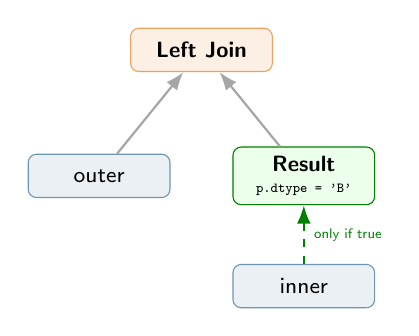
\begin{tikzpicture}[
  joinnode/.style={draw=pgorange!70, rounded corners=3pt, fill=pgorange!12,
               minimum height=0.55cm, minimum width=1.8cm,
               align=center, font=\sffamily\footnotesize},
  tbl/.style={draw=pgblue!70, rounded corners=3pt, fill=pgblue!10,
              minimum height=0.55cm, minimum width=1.8cm,
              align=center, font=\sffamily\footnotesize},
  resultnode/.style={draw=green!50!black, rounded corners=3pt,
               fill=green!8, minimum height=0.55cm, minimum width=1.8cm,
               align=center, font=\sffamily\footnotesize},
  edge/.style={thick, -Latex, gray!70},
  cool/.style={thick, dashed, -Latex, green!50!black},
  saved/.style={font=\sffamily\tiny, text=green!50!black},
]

\node[joinnode] (lj) at (0, 0) {\textbf{Left Join}};

\node[tbl] (outer) at (-1.3, -1.6) {outer};

% Result node injected above inner scan on the inner side
\node[resultnode] (result) at (1.3, -1.6)
  {\textbf{Result}\\[-2pt]{\tiny\texttt{p.dtype = 'B'}}};
\node[tbl] (inner) at (1.3, -3.0) {inner};

\draw[edge] (outer) -- (lj);
\draw[edge] (result) -- (lj);
\draw[cool] (inner) -- node[saved, right, pos=0.5] {\textsf{only if true}} (result);

\end{tikzpicture}

\vspace{1mm}
{\tiny Result node evaluates LHS-only clause as a \textbf{one-time filter}.\\
If false $\to$ returns $\emptyset$; inner scan \emph{never launched}.}
\end{column}

\end{columns}
\end{frame}

% THEORY: One-sided clause guard (from pgsql-hackers thread, Dec 2024)
%
% Each LEFT JOIN's ON clause contains a discriminator predicate that
% depends ONLY on the outer (left) table:
%   LEFT JOIN products p ON ol.item_type = 'product' AND ol.item_id = p.id
%                           ^^^^^^^^^^^^^^^^^^^^^^^^
%                           depends only on ol (outer side)
%
% Currently, the executor evaluates this predicate as a Join Filter
% AFTER probing the inner side.  The inner-side index scan runs
% unconditionally for every outer row -- even when the discriminator
% doesn't match, producing a guaranteed-to-be-rejected result.
%
% The optimization: evaluate the outer-only predicate BEFORE launching
% the inner-side scan.  If it evaluates to false, skip the inner scan
% entirely and immediately emit NULLs for the RHS columns.
%
% Effect on the polymorphic pattern:
%   - Without guard: each row probes ALL N inner sides → N×M total probes
%   - With guard: each row probes only the ONE matching inner side
%     → M total probes (exactly: M_1 + M_2 + ... + M_N = M)
%   - Fruitless probes drop from (N-1)×M to 0
%   - Speedup factor: N (the number of target types)
%
% This is exactly the "plan search-space gap" identified in the chapter:
% no existing plan shape can conditionally skip joins per-row based on
% the discriminator value.  The one-sided clause guard fills that gap
% at the executor level.

\begin{frame}\frametitle{One-Sided Clause Guard}
\vspace{-3mm}
\begin{center}
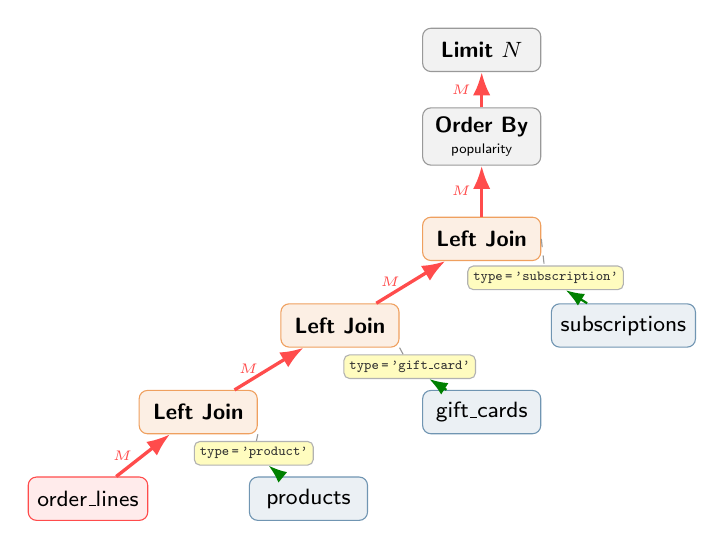
\begin{tikzpicture}[
  joinnode/.style={draw=pgorange!70, rounded corners=3pt, fill=pgorange!12,
               minimum height=0.55cm, minimum width=1.5cm,
               align=center, font=\sffamily\footnotesize},
  tbl/.style={draw=pgblue!70, rounded corners=3pt, fill=pgblue!10,
              minimum height=0.55cm, minimum width=1.5cm,
              align=center, font=\sffamily\footnotesize},
  op/.style={draw=black!40, rounded corners=3pt, fill=black!5,
             minimum height=0.55cm, minimum width=1.5cm,
             align=center, font=\sffamily\footnotesize},
  edge/.style={thick, -Latex, gray!70},
  hot/.style={very thick, -Latex, red!70},
  cool/.style={thick, dashed, -Latex, green!50!black},
  rows/.style={font=\sffamily\tiny\bfseries, text=red!70},
  saved/.style={font=\sffamily\tiny\bfseries, text=green!50!black},
  % Condition tag -- yellow badge connected by dashed line
  cond/.style={draw=black!30, rounded corners=2pt,
               fill=yellow!25, minimum height=0.3cm,
               inner sep=2pt, font=\ttfamily\tiny, text=black!80},
  condline/.style={thin, dashed, black!40},
]

% Row 0: Limit
\node[op] (limit) at (0, 0) {\textbf{Limit $N$}};

% Row 1: Order By (consistent with "Worst case" slide)
\node[op] (orderby) at (0, -1.1) {\textbf{Order By}\\[-2pt]{\tiny popularity}};

% Row 2: Left Join 3
\node[joinnode] (lj3) at (0, -2.4) {\textbf{Left Join}};

% Row 3: Left Join 2 + subscriptions
\node[joinnode] (lj2) at (-1.8, -3.5) {\textbf{Left Join}};
\node[tbl] (t3) at (1.8, -3.5) {subscriptions};

% Row 4: Left Join 1 + gift_cards
\node[joinnode] (lj1) at (-3.6, -4.6) {\textbf{Left Join}};
\node[tbl] (t2) at (0, -4.6) {gift\_cards};

% Row 5: order_lines (red boundary, consistent with "Worst case" slide) + products
\node[tbl, draw=red!70, fill=red!8, align=center] (base) at (-5.0, -5.7)
  {order\_lines};
\node[tbl] (t1) at (-2.2, -5.7) {products};

% Left spine -- still carries M rows (unchanged)
\draw[hot] (base) -- node[rows, left, pos=0.5] {$M$} (lj1);
\draw[hot] (lj1) -- node[rows, left, pos=0.5] {$M$} (lj2);
\draw[hot] (lj2) -- node[rows, left, pos=0.5] {$M$} (lj3);
\draw[hot] (lj3) -- node[rows, left, pos=0.5] {$M$} (orderby);
\draw[hot] (orderby) -- node[rows, left, pos=0.5] {$M$} (limit);

% Inner-side paths: Join --dashed--> [guard badge] <--green-- target table
% The badge sits ON the path as a gate between the join and the inner scan

% Path 1: lj1 --M_1--> [type='product'] <-- products
\node[cond] (c1) at ($(lj1.south east)!0.45!(t1.north west)$)
  {type\,=\,'product'};
\draw[condline] (lj1.south east) -- (c1);
\draw[cool] (t1) -- (c1);

% Path 2: lj2 --> [type='gift_card'] <-- gift_cards
\node[cond] (c2) at ($(lj2.south east)!0.45!(t2.north west)$)
  {type\,=\,'gift\_card'};
\draw[condline] (lj2.south east) -- (c2);
\draw[cool] (t2) -- (c2);

% Path 3: lj3 --> [type='subscription'] <-- subscriptions
\node[cond] (c3) at ($(lj3.east)!0.45!(t3.west)$)
  {type\,=\,'subscription'};
\draw[condline] (lj3.east) -- (c3);
\draw[cool] (t3) -- (c3);

\end{tikzpicture}
\end{center}
\vspace{-3mm}
{\small Guard checks discriminator \emph{before} probing inner side.
Each row probes only the matching table: $M_1\!+\!M_2\!+\!M_3 = M$.}
\end{frame}

\begin{frame}\frametitle{Benefits of the Result Filter Approach}

\begin{itemize}
  \item \textbf{Fewer page accesses.}\;
    Each base row probes only the \emph{matching} inner table instead of
    all~$N$.  Total index/heap page reads drop from $M \times N$ to~$M$.

  \item \textbf{Safety net for missing indexes.}\;
    When no index covers the inner side, the executor would fall back to a
    sequential scan \emph{per outer row}.  The guard lets it skip the scan
    entirely for non-matching rows --- turning an $O(M \times N \times |T_k|)$
    catastrophe into $O(M \times |T_k|)$.
\end{itemize}

\end{frame}

\end{document}
